\documentclass[a4paper,12pt]{book}

% Paquetes necesarios
\usepackage[utf8]{inputenc}   % Codificación de caracteres
\usepackage[spanish]{babel}   % Idioma español
\usepackage[T1]{fontenc}      % Codificación de fuentes
\usepackage{amsmath, amssymb} % Símbolos matemáticos
\usepackage{graphicx}         % Inclusión de gráficos
\usepackage{cite}             % Gestión de citas
\usepackage{hyperref}         % Enlaces y referencias
\usepackage{geometry}         % Configuración de márgenes
\usepackage{fancyhdr}         % Encabezados y pies de página
\usepackage{titlesec}         % Formato de títulos
\usepackage{booktabs}         % Tablas profesionales
\usepackage{caption}          % Personalización de leyendas
\usepackage{enumitem}         % Personalización de listas
\usepackage{float}
\usepackage{tcolorbox}
\usepackage[table]{xcolor} % Paquete para colores en tablas
\usepackage{colortbl}       % Complemento para colorear celdas específicas
\usepackage{multirow}       % Combinar celdas en tablas
\usepackage{makecell}       % Combinar celdas en tablas
\usepackage{enumitem}
\usepackage{amsmath}
\usepackage{eurosym}
\usepackage{tikz}
\usepackage{listings}
\usepackage{color}
\usepackage{float}
\usepackage{pdfpages}
% Configuración de márgenes
\geometry{left=3cm, right=3cm, top=2.5cm, bottom=2.5cm}

% Configuración de encabezados y pies de página
% \setlength{\headheight}{14.49998pt}
\pagestyle{fancy}
\fancyhf{}
\fancyhead[L]{Universidad de Granada}
\fancyhead[L]{\nouppercase{\leftmark}}

% \fancyhead[C]{Escuela Técnica Superior de Ingenierías Informática}
\fancyhead[R]{Fundamentos de Ingeniería del Software}
\fancyfoot[L]{\rule[0pt]{\textwidth}{0.2pt}\\Ismael Sallami Moreno}
\fancyfoot[C]{\rule[0pt]{\textwidth}{0.2pt}\\\thepage}
\fancyfoot[R]{\rule[0pt]{\textwidth}{0.2pt}\\\today}
\renewcommand{\sectionmark}[1]{\markboth{#1}{}} % Configura \leftmark para que solo muestre la sección


% Formato de títulos
\titleformat{\section}{\large\bfseries}{\thesection.}{0.5em}{}
\titleformat{\subsection}{\normalsize\bfseries}{\thesubsection.}{0.5em}{}

% Datos del documento
\title{\textbf{Temario Fundamentos de Ingenierías del Software}}
\author{
    Ismael Sallami Moreno \\
    \texttt{ism350zsallami@correo.ugr.es}
}
\date{
    \vspace{1cm}
    \begin{tabular}{rl}
        \textbf{Asignatura:} & Fundamentos de Base de Datos \\
        \textbf{Tema:} & Teoría \\
        \textbf{Fecha:} & \today
    \end{tabular}
}

\begin{document}

% Portada
\begin{titlepage}
    \begin{center}
        % \vspace*{1cm}
        
        % \Huge
        % \textbf{Práctica Contabilidad Financiera II}
        \Huge \textbf{Temario Fundamentos de Ingeniería del Software} 
        % \vspace{0.5cm}
        % \LARGE
        % \textbf{Ismael Sallami Moreno}\\
        % \LARGE
        % \texttt{ism350zsallami@correo.ugr.es}
        % \LARGE
        % \url{https://github.com/Ismael-Sallami}
        
        % \vfill
        
        % \Large
        % \textbf{Universidad de Granada}
        
        \vspace{0.8cm}
        
        \begin{tikzpicture}[remember picture, overlay]
            \node[opacity=0.2] at (current page.center) {
\includegraphics[width=\paperwidth,height=\paperheight]{portada.jpg}};
            \node[align=center] at (current page.center) {
                
                \vspace{0.5cm}
                \LARGE \textbf{Ismael Sallami Moreno} \\
                \LARGE \texttt{ism350zsallami@correo.ugr.es} \\
                \LARGE \url{https://ismael-sallami.github.io/} \\
                \LARGE \url{https://elblogdeismael.github.io/} \\
                \vspace{2cm}
                \Large \textbf{Universidad de Granada} \\
                \vspace{0.8cm}
                % \Large \textbf{2025}
            };
        \end{tikzpicture}
        \vfill
        
        \Large
        \textbf{2025}
        
    \end{center}
\end{titlepage}
\newpage


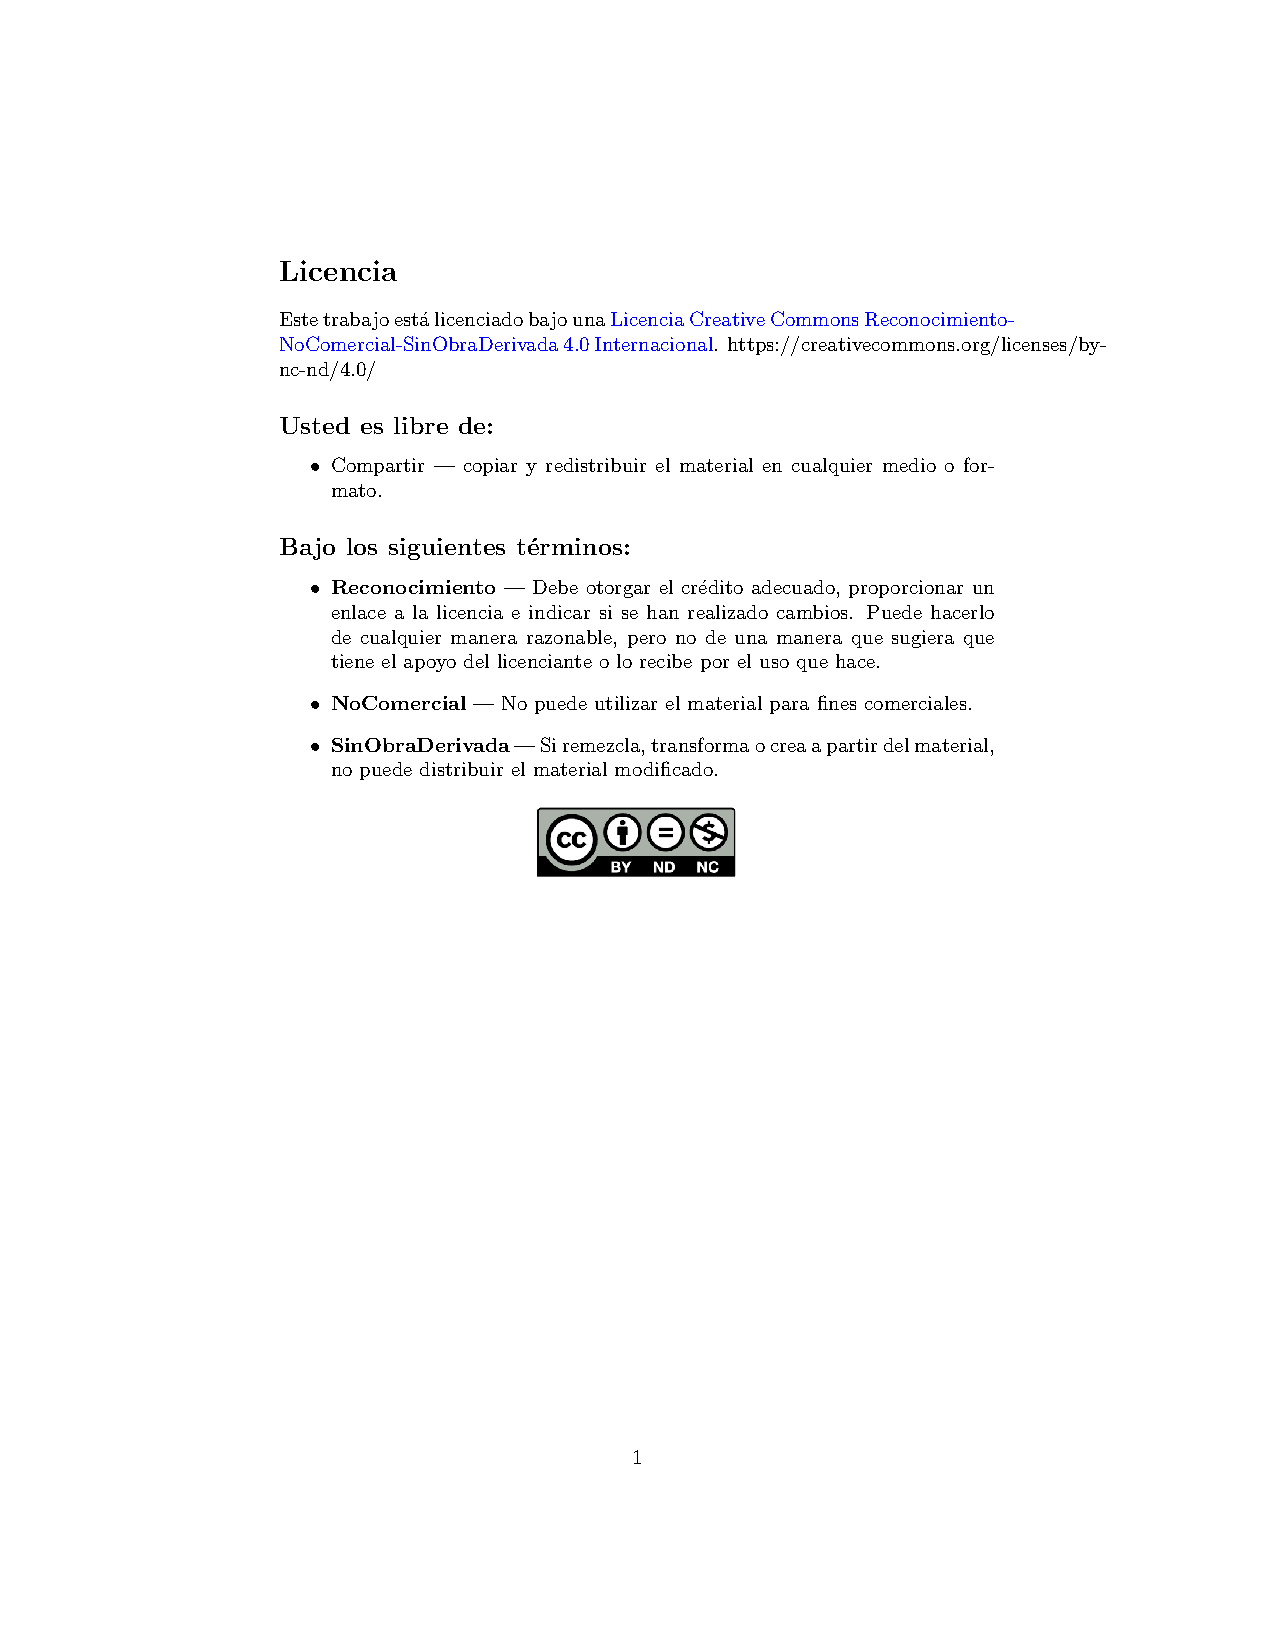
\includepdf[pages=-]{../../../../licencia.pdf}

% Tabla de contenidos
\tableofcontents
\newpage

\chapter{Introducción}

La Ingeniería del Software es una disciplina que se centra en el desarrollo, de coste eficiente, de sistemas software de alta calidad. El software es abstracto e intangible y no se construye con materiales ni se rige por leyes físicas o por procesos de fabricación. De alguna forma, esto simplifica la ingeniería del software ya que no existen limitaciones físicas sobre el potencial del software. Sin embargo, la ausencia de restricciones naturales significa que el software fácilmente puede llegar a ser extremadamente complejo y, por consiguiente, difícil de entender.

En este tema se proporcionará una visión general de las características propias y diferenciadoras del producto software. Se plantearán algunas definiciones del concepto de Ingeniería del Software y, por último, se estudiarán las particularidades específicas del proceso de desarrollo del software.



\includepdf[pages=-,pagecommand={\thispagestyle{fancy}}]{Capitulos/Tema1.pdf}

\chapter{Ingeniería de Requisitos}

Uno de los problemas recurrentes a los que se enfrenta la ingeniería del software es la dificultad para determinar exactamente cuáles son los requisitos de un sistema, es decir, las funcionalidades que debe incluir el sistema a construir, así como todas las consideraciones adicionales sobre seguridad, rendimiento, fiabilidad, cuestiones legales, etc. Y lo que resulta aún más complicado: establecer claramente qué es lo que no debe contemplarse como parte de los requisitos del sistema, bien porque no ha sido incluido en el contrato de desarrollo, o bien porque simplemente queda fuera del alcance del sistema a desarrollar.

La dificultad de la tarea proviene de la dificultad inherente a enunciar, de modo claro y preciso, cualquier problema complejo. Muchos factores afectan negativamente a esta tarea, como por ejemplo el hecho de que los usuarios del futuro sistema pueden no colaborar en la especificación de los requisitos, que los requisitos cambien a lo largo del desarrollo o que aparezcan otros nuevos.

En este tema se planteará qué es la ingeniería de requisitos, se definirá el concepto de requisito y se analizarán los distintos tipos de requisitos y sus propiedades.


\includepdf[pages=-,pagecommand={\thispagestyle{fancy}}]{Capitulos/Tema2.pdf}




\newpage
% Referencias
\begin{thebibliography}{99}
\bibitem{Referencia1}
\emph{Transparencias de la Asignatura de Fundamentos de Ingeniería del Software}, Universidad de Granada, 2025.

\bibitem{Referencia1}
Ismael Sallami Moreno, \textbf{Estudiante del Doble Grado en Ingeniería Informática + ADE}, Universidad de Granada, 2025.


\end{thebibliography}

\end{document}
